%! TeX program = lualatex
%---------------------------ALLGEMEINE IMPORTS-------------------------------------
\documentclass[12pt,english,ngerman]{scrartcl}

\input{./input/shared_preamble.tex}

\addbibresource{opv.bib}
    % Kopfzeile
\ihead{SS22\\04.05.2022}
\chead{\textsc{Hinterleitner} Michael - 12002411 \\ \textsc{Philipp} Maximilian - 11839611}
\ohead{LU ECM-\\ OPV}
    % Fußzeile
%--------------------------------------AB HIER DOKUMENT---------------------------------------------
\begin{document}
\includepdf{deckblatt2.pdf}
\tableofcontents
\newpage


%\section{Aufgabenstellung}\label{sec:Aufgabenstellung}

% Die nachfolgende Aufgabenstellung wurde von den Laborbetreuern bereitgestellt
% und beinhaltet sowohl Angaben zur Vorbereitung als auch zur praktischen
% Durchführung der Übung:

% zu 1: Aufgabenstellung Das vor der Übung verteilte Aufgabenblatt.
 \includepdf[
     pages=-,  % all pages
     addtotoc={
         1, section, 1, Aufgabenstellung, sec:Aufgabenstellung
     }
 ]{angabe.pdf}

% zu 2: Vorbereitung Es sind beide Vorbereitungen dem Protokoll beizufügen.
% \section{Vorbereitung}\label{sec:Vorbereitung}
%Die folgende Vorbereitung wurde vor der Laborübung 
\includepdf[pages=-,
     addtotoc={
         1, section, 2, Vorbereitung, sec:Vorbereitung
     }]{./figures/OpV.pdf}
\includepdf[pages=-]{./figures/Integrator1.pdf}
\includepdf[pages=-]{./figures/Integrator2.pdf}
\includepdf[pages=-]{./mh_vorbereitung_opv.pdf}


% zu 3: Grundlagen In den Grundlagen sollen die später verwendeten Formeln
% stehen und kurz erklärt werden, dabei ist es nicht notwendig Formeln
% herzuleiten. Quellenangaben sind an dieser Stelle von Vorteil, weil Sie so
% schnell die betreffenden Stellen in Unterlagen finden. In den Rechnungen
% werden grundlegende Annahmen skizziert und begründet und dann mit diesen
% Annahmen, die für die Schaltungen notwendigen Werte berechnet. Dabei kann
% auch gleich auf die später wirklich verwendeten Werte Bezug genommen werden -
% wir verwenden bei den Widerständen zum Beispiel von den Normwert-Reihen die
% E12 und/oder E24 Serie (nach DIN 41426 bzw. IEC 63).
\section{Grundlagen}\label{sec:Grundlagen}
%in Grundlagen
Operationsverstärker (kurz 'OPV oder 'OpAmp') dienen der Verstärkung von
Gleichspannungen. Sie besitzen einen nicht-invertierenden, der meist mit einem
Plus gekennzeichnet ist, und einen invertierenden Eingang, der häufigst mit
einem Minus dargestellt wird. Zu beachten ist, dass die Verstärkung auf die
Differenzspannung der beiden Eingänge wirkt. Je zwei zusätzliche Anschlüsse
finden sich für die positive und negative Betriebsspannung und für den
Offsetabgleich, damit bei keiner Eingangsspannung auch keine Ausgangsspannung
auftritt - dieser wird also in einer externen Schaltung durchgeführt.
%In \autoref{fig:pin_anschl} sind die Pins eines Operationsverstärkers, wie er
%auch in der Laborübung verwendet wurde, zu sehen.


Es gibt vier grundlegende Arten der Verwendung von Operationsverstärkern,
darunter der nicht-invertierende Betrieb, bei dem das Eingangssignal nur auf
den nicht-invertierenden Kanal gelegt wird und der invertierende auf Masse
gelegt wird. Analog funktioniert der invertierende Modus, bei dem das Signal
nun an den invertierenden Eingang gelegt wird, wodurch die Ausgangsspannung
zusätzlich zur Verstärkung noch zum Eingangssignal invertiert wird. Beim
Differenzbetrieb werden an beide Eingänge Signale angelegt und die
Differenzspannung verstärkt. Im Falle des Gleichtaktbetriebs liegt das gleiche
Eingangssignal an den beiden Eingängen an, wodurch es theoretisch keine
Differenzspannung und Verstärkung geben sollte - in der Realität resultiert
allerdings eine Verstärkung, die als Gleichtkatkverstärkung bezeichnet wird.

Da der Operationsverstärker ohne zusätzliche Verkopplung sehr stark
frequenzabhängig ist und nur eine geringe Bandbreite gewünscht verstärkt, wird
eine Gegenkopplung vom Ausgang zum Eingang durchgeführt, wodurch die
Verstärkung zwar abnimmt, die Bandbreite jedoch stark vergrößert wird. Die
Bandbreite wird wie gewohnt durch die Grenzfrequenz chraktersisiert, bei
welcher die Verstärkung noch \SI{70}{\%} der maximalen beträgt.

Die resultierende Verstärkung lässt sich gemäß \autoref{eq:ver} als Verhätlnis
der Eingangs- $U_e$ zur Ausgangsspannung $U_a$ berechnen.
%insert eq ---


%in Durchführung
Zu beachten ist, dass jeder nicht belegte Pin auf Massenpotential gelegt wird.


% zu 4: Versuchsdurchführung In diesem Punkt wird die Durchführung der
% einzelnen Aufgaben beschrieben. Im Simulationsteil ist die simulierte
% Schaltung mit allen Analyseparametern darzustellen. Im praktischen Teil sind
% die verwendete Geräte sowie die gemessenen Werte der verwendeten Bauteile
% anzugeben. Außerdem sind durchgeführte Funktionsüberprüfungen der Bauteile
% (Dioden, Transistor, etc.) anzuführen. Die Messergebnisse bzw. Oszillogramme
% sind mit Angabe der verwendeten Messgeräte anzugeben. Oszillogramme werden
% vom verwendeten Oszilloskop als Daten auf einen USB-Stick ausgegeben und
% können in das Protokoll aufgenommen werden. Das gleiche gilt für Schaltungen
% bzw. Ergebnissen von Simulationen. Es ist auf eine klare Darstellung der
% Messergebnisse und –auswertung zu achten (Tabellen, geeignete Grafiken). Die
% originalen, während des Versuchs angefertigten Aufzeichnungen sind dem
% Protokoll beizufügen. 
\section{Versuchsdurchführung}\label{sec:versuchsdurchfuehrung}
Für den praktischen Teil an der Steckplatine wurden Widerstände der E12-Reihe,
mit denen die in der Vorbereitung angegebenen respektive errechneten Werte
angenähert wurden, verwendet. 

Die verwendeten Geräte sind \autoref{tab:geraeteliste} zu entnehmen.

\begin{table}
  \caption{Tabelle der verwendeten Geräte}
  \label{tab:geraeteliste}
  \centering
  \begin{tabular}{l|l}
    \hline
   \multicolumn{2}{ c }{\textbf{Geräteliste}} \\
    \hline
    \textbf{Gerät/Bauelement} & \textbf{Typ} \\
    \hline
    Oszilloskop & \textit{Tektronix TDS 2002}\cite{oszilloscope}\\
    Funktionsgenerator & \textit{H-TRONIC FG250D}\cite{funktionsgenerator} \\
    Netzgerät & nicht bestimmbar\\
    Multimeter & \textit{Fluke 175 TrueRMS}\cite{fluke175} \\
    OPV & \textit{$\mu$A741}\\
    \hline
  \end{tabular}
\end{table}

\subsection{Elektrometerverstärker}

% 5) Die Schaltung ist mit LTspice zu zeichnen und auszudrucken (PDF).
\subsubsection{Simulation} \label{sec:Versuchsim}

% TODO text
Zur Simulation des Elektrometerverstärkers wird das Programm \textit{LTSPICE}
verwendet. Der Aufbau erfolgt analog zum skizzierten Schaltplan in
\autoref{fig:sim_elektrometer_schaltung}. Hier wurde das gleiche Bauteil wie im
Kapitel \nameref{sec:Aufgabenstellung} verwendet, nämlich der $\mu$A741.

\begin{figure}[H]
  \centering
  % TODO LTSPICE aufbau der Elektrometer
    \includegraphics[width=0.95\textwidth]{./figures/elektrometer/sim/sim_schaltung.pdf}
  \caption{Dies ist die Elektrometerverstärkerschaltung; aufgebaut in \textit{LTSPICE}.}
  \label{fig:sim_elektrometer_schaltung}
\end{figure}


% 6) Der Aussteuerungsbereich ist mit einem „DC SWEEP“ zu bestimmen und plotten.
% 7) Anstatt des µA 741 CN, wird in der Simulation das Bauteil LM741 verwendet.
% NEIN fehler in der Angabe sollte UA741 bauteil sein
\paragraph{Untersuchung des Aussteuerungsbereichs} \label{sec:mess_aussteuerungsbereich}

Um den Aussteuerungsbereich zu bestimmen, wurde ein DC-Sweep der
Eingangsspannung durchgeführt und die Ausgangsspannung in Abhängigkeit der
Eingangsspannung graphisch, wie in \autoref{fig:sim_elektrometer_dcsweep}
ersichtlich, dargestellt. Es musste in der Simulation kein
Offsetspannungsabgleich durchgeführt werden.

\begin{figure}[H]
  \centering
  % TODO LTSPICE dc sweep von ausgangsspannung 
    \includegraphics[width=\linewidth, height=7cm]{./figures/elektrometer/sim/aus_sweep.png}
  % TODO check spice directive
  \caption{Die Schaltung aus \autoref{fig:sim_elektrometer_schaltung} wurde auf
    den Aussteuerungsbereich untersucht, indem ein DC-Sweep durchgeführt wurde.
    Hier ist die Ausgangsspannung $VA$ über die Eingangsspannug $V1$
    aufgetragen. Die SPICE-Directive der Simulation ist \texttt{.dc V1 -0.3 0.3 0.01}}
  \label{fig:sim_elektrometer_dcsweep}
\end{figure}

\subsubsection{Steckbrett} \label{sec:elektrometer_steckbrett}
Bevor die Schaltung zunächst aufgebaut werden kann muss die
Funktionstüchtigkeit des OPVs getestet werden, damit keine unzuverlässigen
Komponentten verwendet werden. Daraufhin wird eine Impedanzwandlerschaltung mit
dem funktionstüchtigen OPV gebaut, mit welcher leicht der
Offsetspannungsabgleich gemacht werden kann.


\paragraph{Testschaltung}
% 8) Der Operationsverstärker ist auf seine Funktionstüchtigkeit mit Hilfe der
% vorgegebenen Testschaltung (Invertierender Verstärker) zu überprüfen.
Zur Untersuchung der Funktionstüchtigkeit des OPVs wurde die im Labor vorhandene
Testschaltung, siehe \autoref{fig:testschaltung}, verwendet. 

\begin{figure}[H]
  \centering
  % TODO grafik einfuegen
    \includegraphics[width=0.95\textwidth]{./figures/testschaltung.jpeg}
  \caption{Die vorhandene Testschaltung als invertierender Verstärker.}
  \label{fig:testschaltung}
\end{figure}
% TODO beschreibe wie es angeschlossen wurde

Diese Schaltung wurde verwendet, um zu überprüfen, ob der OPV noch immer die
gewünschten Eigenschaften für positive und negative Verstärkungen aufweist. Dies
wurde durch Variieren des Potentiometers (und somit Variieren der
Eingangsspannung) und dem Messen der Ausgangsspannung erfolgreich überprüft.

% 9) Der Verstärker (bestehend aus OPV, Netzwerk und Spannungsteiler für die
% Eingangsspannung) ist auf dem Steckboard aufzubauen.
\paragraph{Aufbau}
Im Gegensatz zu der in \autoref{fig:sim_elektrometer_schaltung} ersichtlichen
Schaltung wird am Steckbrett ein Spannungsteiler als \SI{100}{mV}
Spannungsquelle verwendet. Dazu wurden ein \SI{15.0}{\kilo\ohm} und ein
\SI{14.96}{\kilo\ohm} mit einem \SI{1}{\kilo\ohm} Poti verwendet um eine wie in
der \autoref{sec:Vorbereitung} ersichtlichen Spannungsteiler zu bauen. Welcher
an der Betriebsspannung $VCC$ \SI{+15}{\volt} und der negativen
Betriebsspannung $VCC-$ \SI{-15}{\volt} anliegt, um eine, durch das dritte
mittelere Bein des Poti abgreifbare, Spannung $V1$ zu erzeugen, welche
mindestens einen, durch das Poti einstellbaren, Bereich von
\SIrange{-500}{500}{\milli\volt} abdecken kann. Weiters wurden die in der
\autoref{fig:sim_elektrometer_schaltung} ersichtlichen Widerstände
\SI{492}{\kilo\ohm} und \SI{7.8}{\kilo\ohm} durch folgende E12-Reihe
Wiederstände \SI{470}{\kilo\ohm} mit \SI{22}{\kilo\ohm} und \SI{6.8}{\kilo\ohm}
mit einem \SI{1}{\kilo\ohm} Poti ersetzt. Das Potentiometer wurde verwendet um
die Ungenauigkeiten der E12 Widerstände beim Verstärkungsfaktor ausbessern zu
können.

\begin{figure}[H]
  \centering
  % TODO Beschriftung der Grafik 
    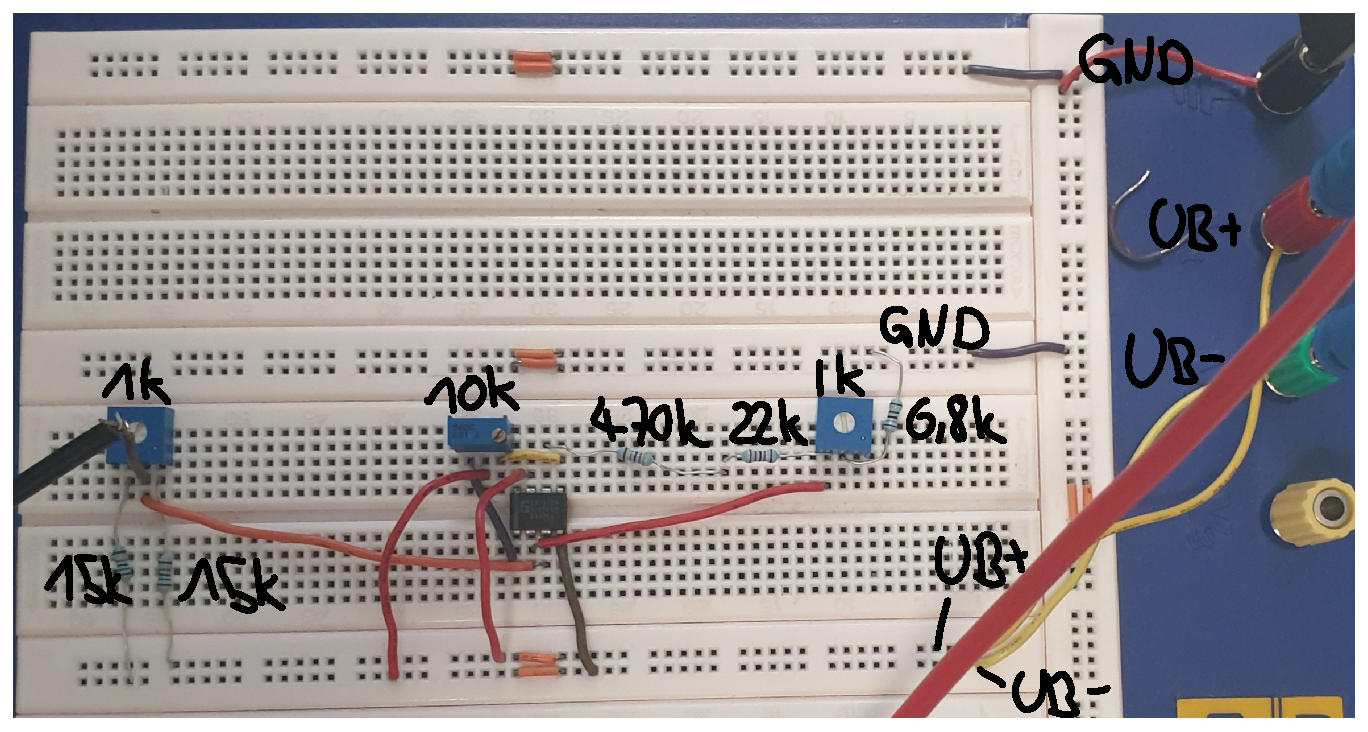
\includegraphics[width=0.95\textwidth]{./figures/elektrometer/steckbrett.png}
  \caption{Der Aufbau des Elektrometerverstärkers am Steckbrett der Schaltung von
  \autoref{fig:sim_elektrometer_schaltung}}
  \label{fig:ver_elektromete_aufbau}
\end{figure}

% 10) Es ist der Offsetspannungsabgleich durchzuführen.
\paragraph{Offsetabgleich}\label{sec:offsetabgleich}
Um den Offsetsspannungableich durchführen zu können, ist zuerst mal ein
Impedanzwandler aufgebaut worden, wodurch das Abgleichen sich zum Abstimmen
der Eingangsspannug zur Ausgangsspannung vereinfachte. Dies wurde durch ein
extern beschaltetes Potentiometer bewerkstelligt, welches die Rolle eines
Spannungteilers spielte. Der Offsetabgleich wurde bei einer Spannung von
\SI{125.4}{\milli\volt} gemacht.

% 11) Die gemessene Ausgangsspannung ist mit der zu erwartenden Ausgangsspannung
% zu vergleichen und das Ergebnis zu protokollieren.
\paragraph{Beschaltung als Elektrometerverstärker}
Nun wurde die Rückkopplung durch einen Spannungsteiler, wie in
\autoref{fig:sim_elektrometer_schaltung} ersichtlich, statt dem Kurzschluss vom
Ausgang zum invertierenden Eingang eingebaut. Zunächst gab es Probleme mit dem
Aufnehmen der Verstärkung, da der Ground einen Wackelkontakt bekommen hat,
welcher durch leichtes drehen des Anschlusses repariert werden konnte.
Nun konnte die $U_a$ und $U_e$ des Elektrometerverstärker gemessen werden. Dies
wurde mittels zwei Multimeter \cite{fluke175} bewerkstelligt, indem wie in
\autoref{fig:sim_elektrometer_schaltung} ersichtlich über die Spannungsquelle
$V1$ und von $VA$ zu Masse gemessen wurde.

Das Potentiometer im Spannungsteiler erlaubte die Verstärkung genau einzustellen.
Jedoch war eine genauere Einstellung schwer per Hand zu bewerkstelligen. Ein digital
ansteuerbares Potentiometer wäre nützlich.

\begin{equation}
  U_a = \SI{8.03}{\volt} \quad @\, U_e = \SI{125.0}{\milli\volt}
  \label{eq:messwert_elektro_ausgang_eingang}
\end{equation}

% 12) Es ist der Aussteuerungsbereich des Verstärkers zu messen.
\paragraph{Untersuchung des Aussteuerungsbereichs} \label{sec:Versuchohnekond}
Um den Aussteuerungsbereich untersuchen zu können wurde der
Eingangsspannugsteiler so dimensioniert, dass dieser an die Grenzen der
Verstärkung des OPVs bis zu der Betriebsspannung treiben kann. Da die
Eingangsspannug von \SIrange{-500}{500}{\milli\volt} liegen kann und der Verstärkungsfaktor
circa \num{64} beträgt ist es leicht bis über die Betriebsspannung hinaus zu
verstärken und dadurch den Aussteuerungsbereich des OPVs durch mehrere
Messungen der Eingangs- $V1$ und Ausgangsspannung $V_a$ untersuchen zu können.


\begin{table}[H]
  \caption{Diese Tabelle beinhaltet die gemessenen Ausgangs- und
    Eingangspannungen der Elektrometerschaltung, welche der Untersuchung des
    Aussteuerungsbereichs eines OPVs\cite{uA741} dienen. Diese Messungen wurden
    unter Verwendung zweier Multimeter\cite{fluke175}, in der
    \autoref{fig:sim_elektrometer_schaltung} ersichtlichen Schaltung, gemacht.
    \\
  $V_a \dots$ Ausgangsspannung \\
  $V1 \dots$ Eingangspannung \\
  }
  \label{tab:mess_elektro_aussteurerung}
  \centering
  \begin{tblr}{SS}
{{{$V1$ / \si{\milli\volt}}}} & {{{$V_a$ / \si{\volt}}}}\\
0.0(2) & 0.0365(3)\\
63.2(3) & 4.082(9)\\
121.5(4) & 7.81(4)\\
180.7(5) & 11.60(4)\\
200.4(6) & 12.86(4)\\
225.2(6) & 13.98(5)\\
244.8(6) & 13.98(5)\\
-62.8(3) & -3.987(8)\\
-117.8(4) & -7.46(4)\\
-176.2(5) & -11.24(4)\\
-233.6(6) & -13.00(4)\\
-290.6(7) & -13.35(5)\\
-298.6(7) & -13.40(5)\\
-340.1(8) & -13.49(5)\\
\end{tblr}

\end{table}


% 13) Die Ergebnisse der Simulation und Messung am Steckboard sind zu diskutieren.

\subsection{Integrator}
% 1) Der Umkehrintegrator ist mit LTspice zu zeichnen und als Abbildung zu speichern.

\subsubsection{Simulation}
Zur Simulation der Integratorschaltung wird das Programm
\textit{LTSPICE} verwendet. Der Aufbau erfolgt analog zum skizzierten
Schaltplan in \autoref{fig:sim_integrator_schaltung}. 

\begin{figure}[H]
  \centering
  % TODO LTSPICE aufbau der Elektrometer
    \includegraphics[width=0.95\textwidth]{./figures/integrator/sim/umkehr_int/schalt_umkehr_100mv.pdf}
  \caption{Dies ist die Integratorschaltung aufgebaut in \textit{LTSPICE}}
  \label{fig:sim_integrator_schaltung}
\end{figure}

% 2) Die Integrationsdauer der Schaltung ist mit einer konstanten Spannungsquelle zu
% simulieren. Die Ergebnisse sind mit der Vorbereitung zu vergleichen.
\paragraph{Integrationszeit}
Um die Integrationszeit, die bei \SI{-10}{\volt} erreicht wird, zu bestimmen,
wurde eine zeitliche Transienten-Analyse durchgeführt, wobei eine konstante
Spannungsquelle von \SI{100}{\milli\volt} verwendet wurde. In
\autoref{fig:sim_integrator_integrationszeit} ist die auftretende
Ausgangsspannung in Abhängigkeit der Zeit zu sehen.

% TODO text

\begin{figure}[H]
  \centering
  % TODO LTSPICE trans anal von lade vorgang 
    \includegraphics[width=\linewidth, height=7cm]{./figures/integrator/sim/umkehr_int/dauer_aussteu.png}
  % TODO check spice directive
  \caption{Die Schaltung aus \autoref{fig:sim_integrator_schaltung} wurde auf
  die Integrationszeit untersucht in dem eine Transiente-Analyse vom
  Ladevorgang gemacht wurde. Die Simulation SPICE-Directive ist \texttt{.tran 0 25 0} 
  bei einer Eingangspannung $V1$ von \SI{100}{\milli\volt}.}
  \label{fig:sim_integrator_integrationszeit}
\end{figure}

\subsubsection{Steckbrett}
% 3) Der OPV ist auf die Funktionstüchtigkeit zu prüfen. (siehe Aufgabe A, Punkt 8)
% 5) Es ist der Offsetspannungsabgleich durchzuführen.
Wie in \autoref{sec:offsetabgleich} erklärt, wurde nochmals mit der
Impdanzwandlerschaltung die Funktionstüchtigkeit überprüft. Ebenfalls wurde
gleich die Offsetabgleich nochmals überprüft. Jedoch musste dieser nicht
angepasst werden, da noch immer alles kalibriert war.

% 4) Der Umkehrintegrator (bestehend aus OPV, Netzwerk und Spannungsteiler) ist auf
% dem Steckboard aufzubauen.
% 6) Die aufgebaute Schaltung ist in Betrieb zu nehmen und die Integrationszeit zu
% protokollieren (Stoppuhr). Die Messung ist fünfmal zu wiederholen.
\paragraph{Integrationszeit}
Nun wurde die charakteristische Ingetrationszeit der Schaltung bestimmt. Indem
zuerst der Kondensator, bis das Multimeter am Ausgang \SI{0}{\mV} anzeigte,
entladen wurde und danach ist die Zeit des Ladens, die die Schaltung brauchte
um die geforderte Spannung von \SI{10}{\volt} am Ausgang zu haben, gemessen.
Dies wurde 6 mal wiederholt um eine Mittelung der Messergebnisse durchführen zu
können.

\begin{table}
  \caption{Messungen der Integrationszeit der realen Integratorschaltung aus
  \autoref{fig:sim_integrator_schaltung}, wobei $T$ die Ladezeit bis am Ausgang
  \SI{10}{\volt} anliegt. Bei einem Ladespannung \SI{91.8}{\milli\volt}, einem
  Widerstand von \SI{21.9}{\kilo\ohm} und einer Kapazität von
  \SI{6.8}{\micro\farad} }
  \label{tab:messungen_integration}
  \centering
  \begin{tabular}[c]{S}
    {$T$ / \si{\second}} \\
    17.20 \\
    16.42 \\
    16.90 \\
    16.89 \\
    17.32 \\
    17.21 \\
  \end{tabular}
\end{table}

% TODO Singale  einfuegen

% 7) Die Schaltung (und Simulation) ist mit verschiedenen Spannungsquellen (Sinus,
% Rechteck, Dreieck) zu testen. Protokollieren und vergleichen Sie die Ergebnisse.
% Nutzen Sie dazu Oszilloskop und Frequenzgenerator.
\paragraph{Untersuchung Verschiedene Eingangssignale}
Nun wurde die Integrationsfähigkeit der Schaltung durch Einspeisen
verschiedener Eingangssignal qualitative untersucht. Dazu wurde zunächst ein
Sinuseingangssignal, siehe \autoref{fig:mess_integrator_sinussignal}, verwendet.
 
\begin{figure}[H]
  \centering
    \includegraphics[width=\linewidth, height=7cm]{./figures/integrator/sinussignal.jpg}
  \caption{Die Aufnahme vom Sinuseingangssignal(Gelb) und dem minus integrieten
  Ausgangssignal (Blau) bei einer Frequenz von \SI{10}{\hertz}. Die
  Einstellungen können dem Oszillogramm direkt entnommen werden.}
  \label{fig:mess_integrator_sinussignal}
\end{figure}

Nun wurde dasselbe mit einem Dreickseingangssignal
, siehe \autoref{fig:mess_integrator_dreiecksignal}, gemacht.

\begin{figure}[H]
  \centering
    \includegraphics[width=\linewidth, height=7cm]{./figures/integrator/dreiecksignal.jpg}
  \caption{Die Aufnahme vom Dreickseingangssignal(Gelb) und dem minus integrieten
  Ausgangssignal (Blau) bei einer Frequenz von \SI{10}{\hertz}. Die
  Einstellungen können dem Oszillogramm direkt entnommen werden.}
  \label{fig:mess_integrator_dreiecksignal}
\end{figure}

Da der Singalgenerator \cite{funktionsgenerator} keine Rechteckspannung erzeugen konnte, konnte
dies auch nicht mit einem Rechteckssignal untersucht werden.

% NOTE: Erwaehnen Rechteckspannung konnte nicht gemacht werden.

% 8) Vergleichen Sie die frequenzabhängige Verstärkung der Schaltung in einem Bereich
% zwischen 5 und 50 Hz mit der Simulation.
\paragraph{Untersuchung der frequenzabhänigen Verstärkung}
Zur Untersuchung der Frequenzabhängigkeit der Verstärkung des OPVs wurde wie im
Kapitel \nameref{sec:Aufgabenstellung} ersichtlich die Frequenz des
Sinuseingangssignals von \SIrange{5}{50}{\hertz} in 15er Schritten varriert.

\begin{figure}[H]
  \centering
    \includegraphics[width=\linewidth, height=7cm]{./figures/integrator/5hz.jpg}
    \caption{In dieser Grafik ist das Sinuseingangssignal(Gelb) bei einer Frequenz von
    \SI{5}{\Hz} und dessen Ausgangssignal(Blau) ersichtlich.}
  \label{fig:mess_integrator_5hz}
\end{figure}

\begin{figure}[H]
  \centering
    \includegraphics[width=\linewidth, height=7cm]{./figures/integrator/20hz.jpg}
    \caption{In dieser Grafik ist das Sinuseingangssignal(Gelb) bei einer Frequenz von
    \SI{20}{\Hz} und dessen Ausgangssignal(Blau) ersichtlich.}
  \label{fig:mess_integrator_20hz}
\end{figure}

\begin{figure}[H]
  \centering
    \includegraphics[width=\linewidth, height=7cm]{./figures/integrator/35hz.jpg}
    \caption{In dieser Grafik ist das Sinuseingangssignal(Gelb) bei einer Frequenz von
    \SI{35}{\Hz} und dessen Ausgangssignal(Blau) ersichtlich.}
  \label{fig:mess_integrator_35hz}
\end{figure}

\begin{figure}[H]
  \centering
   \includegraphics[width=\linewidth, height=7cm]{./figures/integrator/50hz.jpg}
    \caption{In dieser Grafik ist das Sinuseingangssignal(Gelb) bei einer Frequenz von
    \SI{50}{\Hz} und dessen Ausgangssignal(Blau) ersichtlich.}
  \label{fig:mess_integrator_50hz}
\end{figure}


% 9) Die Simulation ist um die genannte Verstärkerstufe zu erweitern.
% Wiederholen Sie mit der neuen Schaltung Punkt 2 und 7
\subsubsection{Simulation des Integrators mit zusätzlicher Verstärkerstufe}

Schlussendlich wird die Integratorschaltung in der Simulation um eine
OPV-Verstärkerstufe gemäß \autoref{fig:sim_integrator_stufe_schaltung}
erweitert, wobei ein zweiter $\mu$A741 als Operationsverstärker in der
Verstärkerstufe verwendet wurde.

\begin{figure}[H]
  \centering
  % TODO LTSPICE aufbau der Elektrometer
    \includegraphics[width=\linewidth]{./figures/integrator/sim/mit_stufe/schaltung_spannungstypen.pdf}
  \caption{Dies ist die Integratorschaltung mit Verstärkerstufe; aufgebaut in \textit{LTSPICE}.}
  \label{fig:sim_integrator_stufe_schaltung}
\end{figure}

Die Integrationszeit, nach welcher die Ausgangsspannung \SI{10}{\volt} beträgt,
wurde erneut graphisch mithilfe einer zeitliche Transienten-Analyse ermittelt,
wobei eine konstante Spannungsquelle von \SI{100}{\milli\volt} verwendet wurde.
Die Ausgangsspannung in Abhängigkeit der Zeit ist in
\autoref{fig:sim_integrator_stufe_integrationszeit} dargestellt.

\begin{figure}[H]
  \centering
  % TODO LTSPICE trans anal von lade vorgang 
    \includegraphics[width=\linewidth, height=7cm]{./figures/integrator/sim/mit_stufe/100mv_aus_zeit.png}
  % TODO check spice directive, pathway
  \caption{Die Schaltung aus \autoref{fig:sim_integrator_schaltung} wurde auf
  die Integrationszeit untersucht, indem eine Transienten-Analyse vom
  Ladevorgang gemacht wurde. Die Simulation SPICE-Directive ist \texttt{.tran 0 16 0} 
  bei einer Eingangsspannung $U_e$ von \SI{100}{\milli\volt}.}
  \label{fig:sim_integrator_stufe_integrationszeit}
\end{figure}

Nun wurden wiederum verschiedene Spannungsquellen als Eingangssignal für den
Integrator mit Verstärkerstufe verwendet. In \autoref{fig:sim_int_stufe_sin}
sind die zeitlichen Verläufe der Eingangs- und Ausgangsspannung bei einem
Sinus-Eingangssignal mit einer Amplitude von \SI{100}{\milli\volt} und einer
Frequenz \SI{5}{\hertz} von ersichtlich. Analog sind Eingangsspannung und
Ausgangsspannung für eine Rechtecksspannung mit einer Amplitude von
\SI{100}{\volt} und einer Periodendauer von \SI{500}{\milli\second} in
\autoref{fig:sim_int_stufe_rect} dargestellt. In
\autoref{fig:sim_int_stufe_tri} sind die Verläufe von $U_e$ und $U_a$ für eine
Dreiecksspannung als Signalquelle zu sehen.
%todo: insert graphs sin, rect, tri

\begin{figure}[H]
  \centering
    \includegraphics[width=\linewidth, height=7cm]{./figures/integrator/sim/mit_stufe/sin100mv_5hz.png}
  \caption{Die Simulation eines Sinuseingangssignal(Pink) und dessen, durch die Schaltung integrieten,
  Ausgangssignal (Grün) bei einer Frequenz von \SI{5}{\hertz}. Die
  Einstellungen können dem Oszillogramm direkt entnommen werden.}
  \label{fig:sim_int_stufe_sin}
\end{figure}

Nun wurde dasselbe mit einem Dreickseingangssignal, siehe
\autoref{fig:mess_integrator_dreiecksignal}, gemacht.

\begin{figure}[H]
  \centering
    \includegraphics[width=\linewidth, height=7cm]{./figures/integrator/sim/mit_stufe/dreieck100mv_500ms.png}
  \caption{Die Simulation eines Dreickseingangssignal(Pink) und dessen, durch die Schaltung integrieten,
    Ausgangssignal (Grün) bei einer Frequenz von \SI{2}{\hertz}. Die
  Einstellungen können dem Oszillogramm direkt entnommen werden.}
  \label{fig:sim_int_stufe_tri}
\end{figure}

\begin{figure}[H]
  \centering
    \includegraphics[width=\linewidth, height=7cm]{./figures/integrator/sim/mit_stufe/rechteck100mv_500ms.png}
  \caption{Die Simulation eines Rechteckseingangssignal(Pink) und dessen, durch die Schaltung integrieten,
  Ausgangssignal (Grün) bei einer Frequenz von \SI{2}{\hertz}. Die
  Einstellungen können dem Oszillogramm direkt entnommen werden.}
  \label{fig:sim_int_stufe_rect}
\end{figure}

% zu 4: Auswertung siehe EPM Skript nur Besprechung von Umformungen und 
% Sachen die man mit den Messungen machen muss damit man Conclusion und Wissen 
% gewinnen kann.
% Entsprechend der in Punkt 2. angegebenen Beziehungen (Formeln) ist aus den
% Messergebnissen in Punkt 5. das in Punkt 1. formulierte Endergebnis zu
% berechnen. Oft ist eine Ermittlung des Endergebnisses aus einer grafischen
% Darstellung bzw. eine grafische Veranschaulichung zweckmaßig. Dabei kann
% die Verwendung von Millimeterpapier oder Computerprogrammen hilfreich sein.
% Wenn eine Bearbeitung der Daten auf dem Computer erfolgt, sollte bei der
% Darstellung der Graphen eine sinnvolle Skalenteilung des Koordinatensystems
% gemacht werden. Die Unsicherheitsbetrachtung f ̈ur die angegebenen Messwerte,
% sowie fur Zwischen- und Endergebnisse ist in diesem Abschnitt
% nachvollziehbar zu beschreiben. Dabei ist nach Kapitel 1 vorzugehen und
% insbesondere auf die Klassifizierung der Unsicherheit (Typ-A/B) und die
% Unsicherheitsfortpflanzung einzugehen.
\section{Auswertung}\label{sec:Auswertung}
% 2) Die Integrationsdauer der Schaltung ist mit einer konstanten Spannungsquelle zu 
% simulieren. Die Ergebnisse sind mit der Vorbereitung zu vergleichen. 
% 3) Der OPV ist auf die Funktionstüchtigkeit zu prüfen. (siehe Aufgabe A, Punkt 8) 
% 4) Der Umkehrintegrator (bestehend aus OPV, Netzwerk und Spannungsteiler) ist auf 
% dem Steckboard aufzubauen.  
% 5) Es ist der Offsetspannungsabgleich durchzuführen. 
% 6) Die aufgebaute Schaltung ist in Betrieb zu nehmen und die Integrationszeit zu 
% protokollieren (Stoppuhr). Die Messung ist fünfmal zu wiederholen. 
% 7) Die Schaltung (und Simulation) ist mit verschiedenen Spannungsquellen (Sinus, 
% Rechteck, Dreieck) zu testen. Protokollieren und vergleichen Sie die Ergebnisse. 
% Nutzen Sie dazu Oszilloskop und Frequenzgenerator. 
% 8) Vergleichen Sie die frequenzabhängige Verstärkung der Schaltung in einem Bereich 
% zwischen 5 und 50 Hz mit der Simulation. 
% 9) Die Simulation ist um die genannte Verstärkerstufe zu erweitern. Wiederholen Sie 


\subsection{Elektrometerschaltung}

\subsubsection{Simulation}
% Verstärkung berechnen

\subsubsection{Verstärkung \& Aussteuerungsbereich}
Damit die Verstärkung in des Elektrometerverstärkers bestimmt werden kann wurde
der lineare Bereich in den Daten aus \autoref{tab:mess_elektro_aussteurerung}
gefittet. Da die Steigung der Vertärkung entspricht wurde diese verwendet  um
die Verstärkung der Schaltung zu finden.

\begin{figure}[H]
  \centering
    \includegraphics[width=\linewidth]{./Output/OPV/opvmessung.png}
    \caption{Diese Grafik zeigt den gemessenen Aussteuerungsbereich des
    $\mu$A741 OPVs. Auf der Ordinaten-Achse befindet sich die Ausgangsspannung
    $V_a$ und auf der Abszisse die Eingangspannung $V1$. Die Daten wurden aus
    \autoref{tab:mess_elektro_aussteurerung} entnommen und als Scatterplot
    dargestellt. Zudem wurde der lineare Operationsbereich des OPVs gefittet um
  die Verstärkung $V$ der realen Elektrometerschaltung genau bestimmen zu
können. Da ein Offset $V_{offset}$ dennoch vorhanden war ist dieser im Fit
berücksichtig worden.}
  \label{fig:gemessene_aussteuerungskurve}
\end{figure}

Die Berechnung und grafische Darstellung wurde mit dem selbstgeschriebenen
Open-Source-Python-Package \texttt{labtool-ex2}\cite{labtool} gemacht. Aus
\autoref{fig:gemessene_aussteuerungskurve} kann die Verstärkung gleich
abgelesen werden, dieser hat einen Wert von \num{64.00(7)}.


\subsection{Umkehrintegrator}

\subsubsection{Integrationszeit}
Die Integrationszeiten aus \autoref{tab:messungen_integration} wurden gemittelt
und dabei wurde die Streuung der Messung als gaußverteilt angenommen.

\begin{equation}
  T = \SI{17.0(4)}{\second}
  \label{eq:wert_integrationszeit}
\end{equation}

% zu 5: Diskussion und Zusammenfassung
% In der Zusammenfassung stehen noch einmal die wichtigsten Messergebnisse, wobei auf Tabellen und
% Abbildungen nur verwiesen werden soll. Die Ergebnisse sind auch zu diskutieren. Insbesondere müssen
% Abweichungen zwischen Simulation und praktischer Durchführung diskutiert werden.
\section{Diskussion und Zusammenfassung}\label{sec:Diskussion} 
\subsection{Diskussion}

\subsubsection{Elektrometerverstärker}
\paragraph{Aussteuerung}
%ausstereung: 0,6-0,9x der Ub sollte Ua bei Aussteuerung max sein -> sättigung
Die Aussteuerung eines Operationsverstärkers soll bei einer Ausgangsspannung
des 0,6 bis 0,9-fachen der Betriebsspannung erreicht werden, was bei einer
Betriebsspannung von \SI{\pm 15}{\volt} eine Spannweite von \SI{\pm 9}{\volt}
bis \SI{\pm 13,5}{\volt} ergibt. Wie in \autoref{fig:sim_elektrometer_dcsweep}
für den Elektrometerverstärker zu sehen, deckt sich dieser Verhalt mit der
Simulation, bei welcher die Aussteuerung ab einer Eingangsspannung von 
\SI{\pm 200}{\milli\volt} auftritt, wobei eine maximale Ausgangsspannung von
\SI{\pm 13}{\volt} erreicht wird. Der Verlauf ähnelt dabei stark der
charakteristischen Kennlinie der Ausgangsspannung eines gewöhnlichen OPVs. Die
Sättigungen im Aussteuerungsbereich, die ebenso bei einer Ausgangsspannung von
\SI{\pm 13}{\volt} erreicht werden, sind auch anhand der Simulationen der
Integrationszeit der Integratorschaltung in
\autoref{fig:sim_integrator_integrationszeit} für die Schaltung ohne respektive
in \autoref{fig:sim_integrator_stufe_integrationszeit} für die Schaltung mit
Verstärkerstufe deutlich zu erkennen. \newline Die Messung der Ausgangsspannung
unter Variation der Eingangsspannung am Steckbrett ergibt, wie in
\autoref{fig:} zu sehen, einen qualitativ sehr ähnlichen Verlauf der
Datenpunkte. 
%todo: insert fig name for scatter plot
Dabei tritt die Sättigung ab einer Eingangsspannung von etwa \SI{\pm
220}{\volt} auf, wobei die maximale Ausgangsspannung auf der positiven Achse
ca. \SI{13,9}{\volt} und auf der negativen \SI{-13,5}{\volt} beträgt. Diese
geringfügigen Abweichungen von der Simulation sind wohl auf das reale Verhalten
der Schaltung (u.a. Temperaturabhängigkeit der Bauelemente) zurückzuführen und
so zu erwarten gewesen.

\paragraph{Ausgangsspannung Steckbrett}
Ziel der Elektrometerverstärker-Schaltung war eine Eingangsspannung von
\SI{125}{\milli\volt} in eine Ausgangsspannung von \SI{8}{\volt} umzuwandeln.
Dies wurde am Steckbrett gemäß \autoref{eq:messwert_elektro_ausgang_eingang}
mit ähnlich hoher Genauigkeit wie bei der Simulation erzielt. Die Abweichung
beträgt demzufolge nur \SI{30}{\milli\volt}, was bei einer Größenordnung von
mehreren Volt vernachlässigbar ist und eine ausreichende Genauigkeit
gewährleistet.

\subsubsection{Integrator}
% 2) Die Integrationsdauer der Schaltung ist mit einer konstanten Spannungsquelle zu 
% simulieren. Die Ergebnisse sind mit der Vorbereitung zu vergleichen. 
\paragraph{Integrationszeit}
Die in der Simulation für den Integrator ohne Verstärkerstufe bestimmte
Integrationsdauer von \SI{15,1}{\second} (siehe
\autoref{fig:sim_integrator_integrationszeit}), die verging bis eine anvisierte
Ausgangsspannung von \SI{-10}{\volt} erreicht wurde, weicht kaum von den Werten
der Vorbereitung (siehe \autoref{sec:Vorbereitung}) ab. Dabei sollte für die
gegebene konstante Spannungsquelle von \SI{100}{\milli\volt} die
Integrationszeit \SI{15}{\second} betragen. Im Rahmen des Versuchs an der
Steckplatine ergab sich bei sechsmaliger Durchführung ein Wert von
\SI{}{\second}.
% TODO discuss the discreptency in the time measurement with the expected result 
%todo: insert int time 
\newline
Für die Integratorschaltung mit Verstärkerstufe sollte gemäß der Vorbereitung
in \autoref{sec:Vorbereitung} bei einer Eingangsspannung von
\SI{100}{\milli\volt} nach \SI{10}{\second} eine Ausgangsspannung von
\SI{10}{\volt} erreicht werden. Mittels der Simulation wurde die
Integrationszeit zu \SI{10,1}{\second} aus
\autoref{fig:sim_integrator_stufe_integrationszeit} bestimmt. Abgesehen von der
erneut nur marginalen Abweichung von \SI{0,1}{\second}, die wohl auf die
Näherungen der Widerstände zurückzuführen ist, impliziert dies, dass die
Schaltung wie geplant funktioniert und erfolgreich konstruiert respektive
dimensioniert wurde.

\paragraph{Spannungsarten}
Die Eingangs- und Ausgangsspannungen für ein Sinussignal sind in \autoref{} für
die Simulation des Umkehrintegrators, in \autoref{} für die Simulation
inklusive Verstärkerstufe und in \autoref{} als Oszillogramm für den
Umkehrintegrator am Steckbrett zu sehen.

\paragraph{Frequenzabhängigkeit}
%frequenzabhängigkeit: opv-schaltung mit rückkopplung; größere variation wäre gut -> bode
%integrationszeit: nahe zielwert, gute Dimensionierung



% TODO discuss the discreptency in the time measurement with the expected result 

%Es wäre wohl vernünftiger gewesen, die Schaltung an der Steckplatine zunächst aufzubauen, um etwaige 
%Ungenauigkeiten durch die Widerstände 
\subsection{Zusammenfassung}

\newpage

\printbibliography

\listoffigures

\listoftables



\end{document}

